\let\negmedspace\undefined
\let\negthickspace\undefined
\documentclass[journal]{IEEEtran}
\usepackage[a5paper, margin=10mm, onecolumn]{geometry}
%\usepackage{lmodern} % Ensure lmodern is loaded for pdflatex
\usepackage{tfrupee} % Include tfrupee package

\setlength{\headheight}{1cm} % Set the height of the header box
\setlength{\headsep}{0mm}     % Set the distance between the header box and the top of the text

\usepackage{gvv-book}
\usepackage{gvv}
\usepackage{cite}
\usepackage{amsmath,amssymb,amsfonts,amsthm}
\usepackage{algorithmic}
\usepackage{graphicx}
\usepackage{textcomp}
\usepackage{xcolor}
\usepackage{txfonts}
\usepackage{listings}
\usepackage{enumitem}
\usepackage{mathtools}
\usepackage{gensymb}
\usepackage{comment}
\usepackage[breaklinks=true]{hyperref}
\usepackage{tkz-euclide} 
\usepackage{listings}
% \usepackage{gvv}                                        
\def\inputGnumericTable{}                                 
\usepackage[latin1]{inputenc}                                
\usepackage{color}                                            
\usepackage{array}                                            
\usepackage{longtable}                                       
\usepackage{calc}                                             
\usepackage{multirow}                                         
\usepackage{hhline}                                           
\usepackage{ifthen}                                           
\usepackage{lscape}
\begin{document}

\bibliographystyle{IEEEtran}
\vspace{3cm}

\title{1.4.9o}
\author{EE24BTECH11011-B.PRANAY KUMAR
}
 \maketitle
% \newpage
% \bigskip
{\let\newpage\relax\maketitle}

\renewcommand{\thefigure}{\theenumi}
\renewcommand{\thetable}{\theenumi}
\setlength{\intextsep}{10pt} % Space between text and floats


\numberwithin{equation}{enumi}
\numberwithin{figure}{enumi}
\renewcommand{\thetable}{\theenumi}




\textbf{Question}:\\
Let \vec{A} \myvec{4\\2}, \vec{B} \myvec{6\\5}, \vec{C} \myvec{1\\4} be the vertices of \(\triangle ABC\). \\
The median from \vec{A} meets \(BC\) at \vec{D}. Find the coordinates of the point \vec{D}.\\
\solution:\\
Using section formula,the mid point of $BC$ is
\begin{align}
\vec{D} &= \frac{\vec{B} + \vec{C}}{2}\\
\end{align}
\begin{align}
    \vec{D} = \myvec{{\frac{7}{2}}\\{\frac{9}{2}}}
\end{align}
Therefore \myvec{{\frac{7}{2}}\\{\frac{9}{2}}} are the required coordinates of \vec{D}.
\begin{figure}[h!]
   \centering
   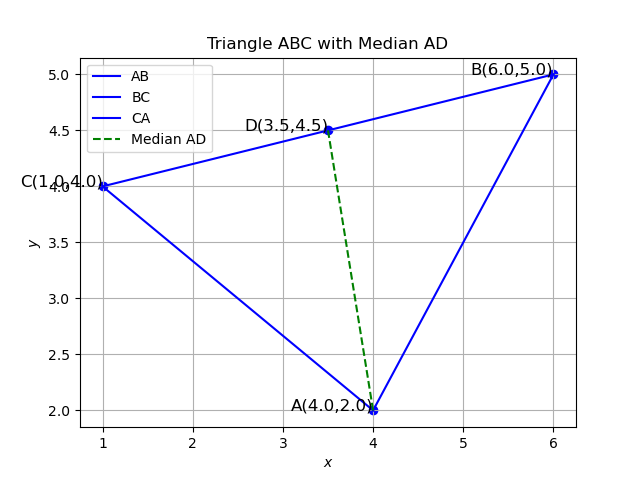
\includegraphics[width=0.7\linewidth]{figs/triangle_plot.png}
   \caption{Median of triangle}
\end{figure}
\end{document}

